%%% -*-LaTeX-*-

\chapter{Two-Dimensional Model of Platelet Rolling}
\label{cha:two-dimens-roll}

\section{The model}
\label{sec:model}

This chapter presents a new model of cell rolling which is similar to
the adhesive dynamics models in that it models bond chemistry as a
stochastic process and computes forces generated by each bond
individually, but simplifies the motion of the cell to translation and
rotation in one dimension, and ignores colloidal forces acting on the
cell. There are two models presented below which rely on the same set
of physical and biological assumptions, described in section
\ref{sec:problem-description}. The deterministic model presented in
section \ref{sec:determ-pde-model} is a mean-field model of platelet
rolling, analogous to the reaction rate equation in chemical kinetics
\cite{Gillespie2007}. The stochastic model presented in section
\ref{sec:stochastic-model} is derived from the same assumptions of the
deterministic model, with the exception that it tracks bonds as
discrete entities which form and break randomly.

\subsection{Problem description}
\label{sec:problem-description}

Below I describe the set of assumptions that we use to model a
platelet translating along an agonist-coated surface. Some important
experimentally variable biological and physical parameters such as
receptor and ligand density, receptor on/off rates, shear rate, and
fluid viscosity appear in the model.

\begin{figure}
  \centering
  \begin{tikzpicture}[scale=3]
  \newcommand{\dist}{0.5}
  \newcommand{\Length}{2.5}
  \newcommand{\slope}{0.5}
  \newcommand{\buff}{0.1}

  % Define a coordinate for the center of the platelet, and draw a
  % node there
  \coordinate (pltcenter) at (0, 1 + \dist);
  \node [circle, inner sep=1.5pt, fill=black] at (pltcenter) {};

  % Draws the wall and the platelet
  \draw (-\Length, 0) -- (\Length, 0);
  \draw (pltcenter) circle [radius = 1];
  \draw[<->] (0, .05) -- node[right] {$\separation$} (0, \dist-.05);
  \draw[<->] (-.15, .05) -- node[left] {$\height$} (-.15,
  .95+\dist);
  \draw[dashed] (0, 1+\dist) -- (-.3, 1+\dist);

  % Draws the lines showing the applied velocities
  \draw[->] (pltcenter) ++(1+\buff, 0) -- node[above] {$\velocity$}
  (\Length-\buff, 1+\dist);

  \draw[->] (0, 1+\dist) ++(135:1+\buff) arc [start angle=135, end
  angle=45, radius=1+\buff] node[midway, above] {$\rotation$};

  % Draws the arrows showing the shear flow
  \foreach \y in {0.5, 1, 1.5, 2, 2.5}
  \draw[->] (-\Length, \y) -- (-\Length + \slope*\y, \y);
  \draw[gray, very thin] (-\Length, 0) -- node[midway, right, black]
  {$V_\tn{fluid} = \shear y$} (-\Length + \slope*\Length, \Length);

  % Draws a bond between the platelet and wall
  \draw[decorate, decoration=zigzag] (pltcenter) ++(315:1)
  node[circle, inner sep=1.5pt, fill=black] {} -- (1.25,0) node
  [circle, inner sep=1.5pt, fill=black] {};

  % Labels the x and theta coordinates
  \draw[{Bar[]}->] (0, -\buff) -- node[fill=white] {$\wallDist$}
  (1.25, -\buff);

  \draw (pltcenter) -- +(0, -1);
  \draw (pltcenter) -- node[above right] {$R$} +(315:1);
  \draw[->] (pltcenter) ++(0, -3*\buff) arc [start angle=270, end
  angle=315, radius=3*\buff] node[midway, below] {$\recAngle$};
\end{tikzpicture}

  \caption[Geometry of the platelet rolling model]{Geometry of the
    platelet rolling model. The platelet is approximated as a sphere
    moving in a 2D shear flow. The reactive region on the platelet
    surface in which receptors on the platelet are close enough to
    ligands on the wall to bind is approximated with a finite
    cylinder. The coordinates $\recAngle$ and $\wallDist$ define the
    platelet and wall attachment points of a bond.}
  \label{fig:model-geometry}
\end{figure}

\subsubsection{Geometry and physics}
\label{sec:geometry-physics}

A sketch of the problem geometry is given in Figure
\ref{fig:model-geometry}. Assume we have a circular rigid platelet (of
radius $\radius$) rolling and translating in shear flow with shear
rate $\shear$ adjacent to a wall. The platelet translates parallel to
the wall at speed $\velocity$, and rolls at angular velocity
$\rotation$. Because the circle is always translating parallel to the
wall, there is a fixed vertical distance $\separation$ between the
wall and the closest point on the circle. Define the height $\height$
of the platelet to be the distance from the wall to the center of the
platelet ($\height = \separation + \radius$). The fluid forces exerted
on the platelet are a function of $\height$, $\radius$, $\shear$, and
$\velocity$, as well as the fluid viscosity ($\viscosity$) which is
constant across all experiments. We assume that the platelet is moving
in a Stokes flow, meaning that inertial forces are negligible and
force balance must be satisfied on the platelet at all times.

Due to the linearity of Stokes equations:
\begin{align}
  \label{eq:stokes-momentum}
  0 &= -\nabla p + \mu\Delta \mathbf{u} + \mathbf{F}\\
  \label{eq:stokes-mass}
  0 &= \nabla \cdot \mathbf{u},
\end{align}
there is a linear relationship between platelet velocity and drag
force from the fluid acting on the platelet. In a 3D Stokes flow, this
relationship is given by a $6 \times 6$ matrix equation
$\mathbf{F}_\tn{drag} = \underline{\underline{R}} \mathbf{U}$ where
$\mathbf{U}$ is a $6 \times 1$ vector containing the 3 translational
velocities and 3 rotational velocities, and $\mathbf{F}$ is a
$6 \times 1$ vector containing the 3 forces and 3 torques. However in
the current model we have made a number of simplifying assumptions.
\begin{enumerate}
\item We assume the flow is a 2D Stokes flow, eliminating all forces
  and translational velocities along the dimension going into and out
  of the page. This also eliminates rotations and torques about the
  two dimensions on the page. Similarly the platelet geometry is a
  circle in 2D. We arrive at this assumption by assuming the platelet
  is a sphere in 3D, but due to the length-dependence of bond
  formation and breaking there is only a narrow reactive strip of
  width $\width$ along the bottom of the platelet in which bonds
  exist. We then approximate this narrow reaction region with a finite
  cylinder of height $\width$ and radius $\radius$.
\item The platelet remains at a constant separation distance from the
  wall, eliminating all vertical motion (and consequently ignoring all
  vertical forces imposed by bonds between the platelet and wall). In
  published adhesive dynamics models, the nonspecific repulsive forces
  between the platelet and vessel wall are only significant at very
  short ranges, therefore it is plausible that at the length scales
  relevant to the problem, the height of the platelet from the surface
  does not change, and bond forces pulling the platelet towards the
  wall are balanced by the nonspecific repulsive forces.
\item The hydrodynamic forces on the platelet are computed assuming
  the platelet is infinitely far from the wall. In particular the
  translational velocity of the platelet is assumed to be independent
  of the torque, and vice versa. This assumption is nonphysical,
  however it does simplify the relationship between bond forces and
  torques and the platelet translation and angular velocities. In the
  near future, I will remove this assumption and instead use the
  formulae of Goldman, Cox, and Brenner
  \cite{Goldman1967a,Goldman1967b} to find the drag force on the
  platelet (see section \ref{sec:height-depend-fluid}).
\end{enumerate}
With these assumptions in place, the force balance condition reduces
to two decoupled linear equations relating the horizontal force
($\horzTotalForce$) to the translational velocity ($\velocity$) and
relating the torque ($\totalTorque$) to the rotational velocity
($\rotation$):
\begin{align}
  \label{eq:force-bal}
  0 &= \velFriction(\appliedVel - \velocity) + \horzTotalForce \\
  \label{eq:torque-bal}
  0 &= \rotFriction(\appliedRot - \rotation) + \totalTorque
\end{align}
% Equations.
% NOTE: I will need to expand on this more when I add equations to
% the paper. I also forgot to discuss the applied fluid velocities.

We identify bonds by their two attachment points on the wall and on
the platelet surface, so each bond has two coordinates associated with
it for each of its endpoints. Points on the wall are given by the
coordinate $\wallDist$, defined to be the horizontal distance from the
center of the circle, and points on the platelet surface are given by
the coordinate $\recAngle$, defined to be the angle formed by the
receptor, the center of the circle, and the closest point on the
circle to the wall (Figure \ref{fig:model-geometry}). With this
definition of $\wallDist$ and $\recAngle$, the distance from a ligand at
$\wallDist$ on wall and a receptor $\recAngle$ on the platelet surface is
given by the equation
\begin{equation}
  \label{eq:dim-length}
  \length^2 (\wallDist, \recAngle) \equiv (\radius - \radius\cos\recAngle +
  \separation)^2 + (\radius\sin\recAngle - \wallDist)^2.
\end{equation}

\subsubsection{Biology}
\label{sec:biology}

The platelet surface is covered with receptors at an angular density
of $\receptorDensity$ receptors/radian, and bonds can form between
points on the surface of the circle and points on the wall. The number
of ligand binding sites on the substrate is assumed to be in
excess. We assume that bonds act like Hookean springs with a rest
length of 0, so the force exerted by a bond is proportional to its
length and the proportionality constant is the stiffness of the
bond. Formation and dissociation rates are distance and force
dependent, respectively. We use the Bell model \cite{Bell1978} to
express the bond dissociation rate as a function of force. The bond
formation rate comes from assuming that the binding site on the ligand
is normally distributed in space, therefore the bond formation rate is
proportional to a Gaussian function of bond length. Therefore the
equations for formation rate and dissociation rate are the following:
\begin{align}
  \label{eq:binding}
  \onRate(\length) &= \onConst \exp
                     \left(-\frac{\stiffness}{2\boltzmann\temp}
                     \length^2(\wallDist, \recAngle) \right), \\
  \label{eq:unbinding}
  \offRate(\length) &= \offConst \exp \left( \frac{\stiffness
                      \length(\wallDist, \recAngle)}{\refForce} \right).
\end{align}

In order to calculate $\horzForce$ and $\torque$ for an existing set
of bonds between the platelet and wall, we simply have to add up the
individual contributions to the force and torque from each bond. The
force and torque generated by an individual bond can be derived from
the geometry of the model along with the assumption that the force
vector $\mathbf{F}$ points in the same direction as the bond with
magnitude proportional to the bond length. The horizontal force
generated by a single bond ($\horzForce$) is given simply by
\begin{equation}
  \label{eq:horz-force}
  \horzForce = \stiffness (\wallDist - \radius\sin\recAngle),
\end{equation}
while the torque generated by a single bond ($\torque$) is given by
the somewhat more complicated
\begin{equation}
  \label{eq:torque}
  \torque = -\stiffness \radius ((\radius - \radius\cos\recAngle +
  \separation)\sin\recAngle + (\radius\sin\recAngle -
  \wallDist)\cos\recAngle).
\end{equation}

\subsection{Deterministic PDE model}
\label{sec:determ-pde-model}

If we assume that there is a continuous distribution of bonds between
the platelet and the wall, we can define the function
$\bondDensity(\wallDist, \recAngle, \dTime)$ which gives the density of
bonds at time $\dTime$ between points $\wallDist$ and $\recAngle$ on the
wall and platelet, respectively. Bonds advect in $\wallDist$ with
velocity $\velocity$ and they advect in $\recAngle$ with velocity
$\rotation$. Bonds form at the rate given in equation
(\ref{eq:binding}) and saturate in $\recAngle$ with a maximum density
$\receptorDensity$. Finally, bonds break at the force-dependent rate
given in equation (\ref{eq:unbinding}). Putting all of this together
gives us the following PDE definition of $\bondDensity$:
\begin{equation}
  \label{eq:bond-density}
  \Pder{\bondDensity}{\dTime} = \rotation
  \Pder{\bondDensity}{\recAngle} + \velocity
  \Pder{\bondDensity}{\wallDist} + \onRate(\length)
  \left(\receptorDensity - \DimReceptorSaturation \right) -
  \offRate(\length) \bondDensity(\wallDist, \recAngle, \dTime).
\end{equation}

This equation can't yet be solved for $\bondDensity$, because there
are still 2 unknowns in it: $\velocity$ and $\rotation$. Recall from
above that $\velocity$ and $\rotation$ are found by balancing the
fluid and bond forces acting on the platelet (equations
(\ref{eq:force-balance}) and (\ref{eq:torque-balance})). First, we
have to calculate the total force $\horzTotalForce$ and torque
$\totalTorque$ generated by the distribution of bonds $\bondDensity$:
\begin{align}
  \label{eq:horz-total-force}
  \horzTotalForce &= \DimQuantity{\horzForce}, \\ 
  \label{eq:total-torque}
  \totalTorque &= \DimQuantity{\torque}
\end{align}

Once we have $\horzTotalForce$ and $\totalTorque$, the platelet velocities
$\velocity$ and $\rotation$ are given by the equations:
\begin{align}
  \label{eq:force-balance}
  0 &= \velFriction (\appliedVel - \velocity) + \horzTotalForce, \\
  \label{eq:torque-balance}
  0 &= \rotFriction (\appliedRot - \rotation) + \totalTorque.
\end{align}

Now we have 3 equations in 3 unknowns and this is a closed system that
can be solved simultaneously for $\bondDensity$, $\velocity$, and
$\rotation$. We still need to define the domains of all three
variables, and give boundary conditions for $\bondDensity$ before we
can solve this system. Assume that bonds can only attach to the lower
half-circle of the platelet surface, while bonds can form at any point
along the wall. Thus we are solving $\bondDensity$ in the domain
$(-\infty, \infty) \times [-\pi/2, \pi/2]$. We need to enforce
boundary conditions at the upstream (with respect to variables
$\wallDist$ and $\recAngle$) ends of the $\wallDist$ and $\recAngle$
domains. Because we assume there are no bonds attached to the upper
half of the platelet, and because the equilibrium concentration of
bonds $\bondDensity \rightarrow 0$ as $L \rightarrow \infty$, we must
set homogeneous Dirichlet boundary conditions on both $\wallDist$ and
$\recAngle$. Finally we set the initial condition to be
$\bondDensity(\wallDist, \recAngle, 0) \equiv \bondDensity_0(\wallDist,
\recAngle)$.

In order to eliminate some parameters, we nondimensionalize this model
by introducing nondimensional coordinates
$\wallDist = \radius \ndWallDist$ and $\ndTime = \offConst \dTime$
(note that $\recAngle$ is already dimensionless) and nondimensional
functions $\radius \bondDensity = \receptorDensity \ndBondDensity$,
$\velocity = \radius \offConst \ndVelocity$, and
$\rotation = \offConst \ndRotation$. The details of the
nondimensionalization are included in Appendix \ref{app:nondim}, but
the final nondimensional set of equations is
\begin{align}
  \nonumber
  \Pder{\ndBondDensity}{\ndTime}
  &= \ndRotation \Pder{\ndBondDensity} {\recAngle} + \ndVelocity
    \Pder{\ndBondDensity}{\ndWallDist} + \ndOnConst \exp
    \left(-\frac{\onForceScale}{2} \ndLength^2(\ndWallDist, \recAngle)
    \right) \left(1 - \NDReceptorSaturation\right) \\
  \label{eq:nd-bond-density}
  &\qquad - \exp
    \left(\offForceScale\ndLength(\ndWallDist, \recAngle)\right)
    \ndBondDensity(\ndWallDist, \recAngle, \ndTime), \\
  \label{eq:nd-force-balance}
  0 &= \ndVelFriction \left(\ndAppliedVel - \ndVelocity\right) + 
      \ndHorzTotalForce, \\
  \label{eq:nd-torque-balance}
  0 &= \ndRotFriction \left(\ndAppliedRot - \ndRotation\right) +
      \ndTotalTorque.
\end{align}

The nondimensional bond length $\ndLength$ is given by
\begin{equation}
  \label{eq:nd-length}
  \ndLength^2(\ndWallDist, \recAngle) = (1 - \cos\recAngle +
  \ndSeparation)^2 + (\sin\recAngle - \ndWallDist)^2,
\end{equation}
and the nondimensional force $\ndHorzTotalForce$ and torque
$\ndTotalTorque$ are given by
\begin{align}
  \label{eq:nd-force}
  \ndHorzTotalForce &= \NDQuantity{(\ndWallDist - \sin\recAngle)} \\
  \label{eq:nd-torque}
  \ndTotalTorque &= \NDQuantity{\left[ \left(1 - \cos\recAngle +
                   \ndSeparation\right) \sin\recAngle +
                   \left(\sin\recAngle - \ndWallDist\right)
                   \cos\recAngle \right]}
\end{align}
A complete list of the nondimensional coordinates, functions, and
parameters with their definitions are given in Table
\ref{tab:nd-vars}.

\subsection{Stochastic model}
\label{sec:stochastic-model}

An assumption that is implicit in the deterministic model is that cell
rolling is mediated by a large number of bonds between the platelet
and the surface, and therefore by the law of large numbers randomness
of bond formation and breaking is inconsequential. This assumption is
not supported by previous rolling models, nor is it supported by
experimental observation. In \cite{Wang2013}, which models platelet
rolling along vWF, at no point during their numerical experiment does
the number of bonds between the platelet and surface exceed 9. Even in
models of leukocyte rolling, where the drag force on the cell is
several times greater than drag on a platelet, the number of bonds
between the cell and the surface is approximately 20 at any given
point in time.

Therefore, there is good evidence that rolling is mediated by a small
number of bonds that can halt a platelet, and the implicit assumption
in the deterministic model that there are many bonds is not valid. In
order to fully and accurately describe platelet rolling, we must model
bond formation and breaking as a stochastic process, and consequently
the rolling velocity of the platelet is a stochastic process.

\subsubsection{Assumptions in the stochastic model}
\label{sec:assumpt-stoch-model}

For the stochastic model---like the deterministic model---assume that
there are $\receptorDensity$ receptors per radian, and the receptors
are uniformly distributed along the surface of the platelet. Assume
there is an excess of ligand on the wall surface, so that bonds can
form anywhere along the wall and there is no saturation of bonds in
the $\wallDist$ dimension.

A bond can form between a receptor located at $\recAngle$ and a point
$\wallDist$ on the wall at ``rate'' $\onRate(\wallDist,
\recAngle)$. More precisely, the time $t_\tn{form}$ that it takes a
bond to form between $\wallDist$ and $\recAngle$ is exponentially
distributed with mean $1/\onRate(\wallDist, \recAngle)$. Similarly,
the time it takes a bond between $\recAngle$ and $\wallDist$ to break
is exponentially distributed with mean
$1/\offRate(\wallDist, \recAngle)$. Finally, a single bond between
$\wallDist$ and $\recAngle$ generates horizontal force and torque
which are given by $f_h$ and $\tau_s$ as defined in equations
(\ref{eq:horz-force}) and (\ref{eq:torque}). As in the continuous
model, assume that only bonds on the lower half-circle of the platelet
can interact with the wall surface.

One consideration that we must make in the stochastic model is how to
handle bond saturation. The PDE enforces a maximum bond density on the
surface of the platelet, but bond density does not make sense in the
stochastic model because bonds are discrete in this model. One
approach is tracking every receptor on the surface of the platelet---
bound or unbound---and assuming that each receptor can only form a
single bond. But there are thousands of receptors on a platelet
surface, and it is inefficient to track all of them and calculate bond
formation rates for all of them. A more flexible approach is described
below, which groups receptors into bins that move with the surface of
the platelet. This is just a generalization of the approach of
tracking each receptor individually: taking the number of bins
equal to the number of receptors reduces to the case of tracking each
receptor individually.

At the beginning of a simulation, I partition the entire platelet
surface $\theta \in [-\pi, \pi)$ into $2N$ subintervals of equal
length
$I_j(0) = \left[-\frac{\pi}{2} + \frac{\pi}{N}j, -\frac{\pi}{2} +
  \frac{\pi}{N} (j+1)\right)$. Each subinterval has width
$\nu \equiv \pi/N$. Within each subinterval $I_j$, there are
$b_\tn{max} \equiv \receptorDensity \pi/N$ total receptors, which are
all assumed to be located at the midpoint $\binMidpoint{j}$ of the
interval:
$\binMidpoint{j}(0) \equiv -\frac{\pi}{2} + \frac{\pi}{N} \left( j +
  \frac{1}{2} \right)$. As the simulation evolves, the intervals $I_j$
(and their midpoints $\binMidpoint{j}$) track with the surface of the
platelet as it rotates; that is, they form a Lagrangian partition of
the platelet surface (see Figure \ref{fig:plt-bins}).

\begin{figure}
  \centering
  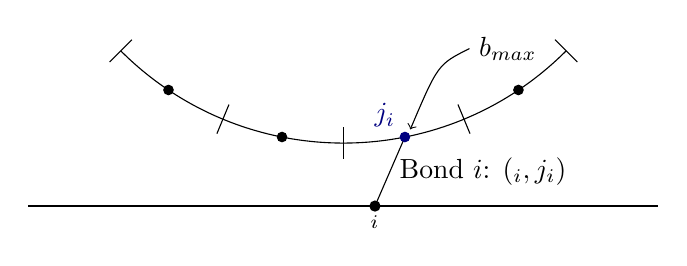
\begin{tikzpicture}
  [scale=4,
  midpoints/.style=blue!50!black,
  intervals/.style=red!50!black]
  \draw (225:1) arc [start angle=225, end angle=315, radius=1];
  \foreach \th in {-2,...,2}
  \draw (270 + 22.5*\th:.95) -- (270 + 22.5*\th:1.05);

  \draw[semithick] (-1, -1.2) -- (1, -1.2);
  \draw (281.25:1) -- node[right] {Bond $i$: $(\wallDist_i, j_i)$}
  (.1, -1.2);
  \filldraw[semithick] (.1, -1.2) node[below] {$\wallDist_i$} circle
  [radius=.015];
  
  \foreach \th in {236.25,258.75,303.75}
  \filldraw (\th:1) circle [radius=.015];
  
  \filldraw[midpoints] (281.25:1) node [above left] {$\binMidpoint{j_i}$}
  circle [radius=.015];

  \draw[->] (.4,-.7) node [right] {$b_\tn{max}$}
  .. controls (.3, -.75) .. (282.5:.98);
\end{tikzpicture}

  \caption[Partition of (part of) the platelet surface into
  $\recAngle$-bins.]{Partition of (part of) the platelet surface into
    $\recAngle$-bins. There are $b_\tn{max}$ total receptors in each
    $\recAngle$-bin, and they are all assumed to be located at the
    midpoint of the interval.}
  \label{fig:plt-bins}
\end{figure}

\subsubsection{A modified Gillespie algorithm}
\label{sec:modif-gill-algor}

In order to simulate the random bond breaking and formation, we have
to take into account the motion of the platelet as well as the
reaction rates for each possible binding/unbinding reaction. Because
every reaction has a spatially varying reaction rate and the platelet
is moving, each reaction rate changes over time. A naive way to
approach this is to modify the Gillespie algorithm by enforcing some
maximum time step, and if no reaction occurs within the maximum
allowed time step, update the position of the platelet without
creating any new bonds or destroying any existing ones. For now this
is our chosen approach, but a more efficient method for simulating the
stochastic model is developed in section \ref{sec:modif-next-react}

To summarize the current stochastic simulation method, each time step
begins by calculating the rates of all possible reactions. The
possible reactions are either the formation of a new bond from 1 of
the $N$ subintervals on the lower half of the platelet, or the
breaking of any existing bonds. Then two random numbers are generated
to choose the time $\Delta t$ until the first reaction and which
reaction occurred. The propensity for a bond of nondimensional length
$\ndLength$ to break is given by
$\exp(\offForceScale \ndLength(\ndWallDist, \recAngle))$, and the
propensity for a new bond to form from subinterval $j$ to \emph{any}
point on the wall is given by
$b_j^\tn{avail} \ndOnConst\Int{\exp\left(-\onForceScale \ndLength^2
  (\ndWallDist, \recAngle)/2\right)} {\ndWallDist} {-\infty} {\infty}$
although in practice this integral is truncated for consistency with
the deterministic model. The number of available receptors
$b_j^\tn{avail}$ in interval $I_j$ is given by $b_\tn{max} - n_j$
where $n_j$ is the number of receptors occupied by existing bonds.

If the chosen maximum time step $\Delta t_\tn{max}$ is smaller than
the time to the next reaction $\Delta t$, then no reactions occur and
the platelet position is updated. If $\Delta t < \Delta t_\tn{max}$,
update the position of the platelet and then update the bond list
based on which reaction occurred. If a bond is chosen to break, that
bond is simply removed. If a new bond is chosen to form from position
$\binMidpoint{j}$ on the platelet, then a point on the wall must be
selected to attach the bond to. This is described in more depth
below. Once the bond list is updated, new bond forces and torques are
calculated, and new velocities $\ndVelocity$ and $\ndRotation$ are
found. This process then repeats until the end of the simulation is
reached.

\paragraph{Bond formation}
\label{sec:bond-formation}

As mentioned above, the propensity of bond formation from a point
$\binMidpoint{j}$ on the platelet to any point on the wall is the
integral over $\ndWallDist$ of the bond formation rate:
\begin{equation}
  \label{eq:new-bond-prop}
  a_j = b_j^\tn{avail} \ndOnConst \Int{\exp \left(-\frac{\onForceScale}{2}
      \ndLength^2 (\ndWallDist, \binMidpoint{j}) \right)} {\ndWallDist}
  {-\infty} {\infty}.
\end{equation}

Suppose a new bond is guaranteed to form with a platelet attachment
point $\binMidpoint{j}$. Then by reasoning similar to that used to
choose the next reaction in Gillespie algorithm, the probability that
the wall attachment point of that bond is in some interval
$[\ndWallDist_1, \ndWallDist_2]$ is just the proportion of the overall
integral (\ref{eq:new-bond-prop}) contained in that interval:
\begin{equation}
  \label{eq:wall-cum-dist}
  \mathbb{P} \left[\ndWallDist_\tn{new} \in [\ndWallDist_1,
    \ndWallDist_2] \right] = \frac{b_j^\tn{avail} \ndOnConst \Int{\exp
      \left( -\frac{\onForceScale}{2} \ndLength^2(\ndWallDist,
        \binMidpoint{j}) \right)} {\ndWallDist} {\ndWallDist_1}
    {\ndWallDist_2}} {a_j}.
\end{equation}
From equation (\ref{eq:wall-cum-dist}), the wall attachment point
$\ndWallDist_\tn{new}$ of the new bond is normally distributed:
\begin{equation}
  \label{eq:wall-dist}
  \ndWallDist_\tn{new} \sim \mathcal{N}\left( \mu =
    \sin(\binMidpoint{j}), \sigma^2 = \onForceScale\inv \right).
\end{equation}
Therefore when a new bond forms, the platelet attachment point of the
bond is selected using the overall propensity $a_j$ and the wall
attachment point is chosen from the normal distribution
(\ref{eq:wall-dist}) after $\binMidpoint{j}$ is chosen.

In practice the $\ndWallDist$ coordinates are restricted to finite
values. While there is no practical need to do this, it ensures
consistency with the deterministic algorithm where extending the
domain of $\ndWallDist$ to $\reals$ is not possible.

\subsubsection{Some implementation details}
\label{sec:some-impl-deta}

The stochastic simulation algorithm is described in detail in Appendix
\ref{cha:numerical-schemes}; here I outline the algorithm and mention
some of the important implementation details. Just like the
deterministic algorithm, the stochastic algorithm tracks 3
time-varying unknowns: bonds between the platelet and wall,
translational velocity, and angular velocity. However now the bonds
between the platelet and surface are tracked discretely, and the
number of bonds between the platelet and wall follows a stochastic
process. Both velocities are stochastic processes as well, because of
their dependence on the bonds between the platelet and wall.

Key features of the algorithm are as follows:
\begin{enumerate}
\item Platelet-wall bonds are tracked in an array which stores the two
  endpoints of each bond. Each row represents a single bond; the first
  column stores the $\ndWallDist$ coordinate of the bond (the wall
  attachment point), and the second column stores $j$ (the
  $\recAngle$-bin from which the bond formed.
  \begin{equation}
    \label{eq:bond-list}
    \texttt{bondList} =
    \begin{bmatrix}
      \ndWallDist_0 & j_0 \\
      \ndWallDist_1 & j_1 \\
      \vdots & \vdots \\
      \ndWallDist_{\texttt{numBonds}-1} & j_{\texttt{numBonds} - 1}
    \end{bmatrix}    
  \end{equation}
  where $j_i = 0, \hdots, 2N-1$ and
  $\Der{\ndWallDist_i}{\ndTime} = -\ndVelocity(\ndTime)$ for
  $i = 0, \hdots, \texttt{numBonds} - 1$.

  As time evolves, $\texttt{bondList}$ is updated in two ways: (1) the
  $\ndWallDist$-coordinate changes as the platelet moves, and (2) rows
  are added to or removed from $\texttt{bondList}$ as bonds form or
  break.
\item Values for $\binMidpoint{j}$ are tracked in an array which gets
  updated every time step:
  \begin{equation}
    \label{eq:midpt-list}
    \texttt{midpoints} = \left[\binMidpoint{0}, \binMidpoint{1}, \hdots,
      \binMidpoint{2N - 1}]\right.
  \end{equation}
  The update for each step is
  $\texttt{midpoints} = \texttt{midpoints} + \omega$ where $\omega$ is
  the rotation rate for the current time step.
\item Each time step consists of the following:
  \begin{enumerate}
  \item Calculate the reaction propensities
  \item Find the time to the next reaction and which reaction occurs
  \item Update the bond positions in $\texttt{bondList}$ and
    $\texttt{midpoints}$, and then add/remove a bond to/from
    $\texttt{bondList}$ if necessary
  \item Calculate the new forces and torques
  \item Find the new rolling velocities $\ndVelocity$ and $\ndRotation$.
  \end{enumerate}
\end{enumerate}

\section{Results and Analysis}
\label{sec:results}

The model described above is a fairly simple model of platelet
rolling. The geometry of a platelet is greatly idealized, the
hydrodynamic and chemical forces between the platelet and surface are
simplified, and platelet activation is not considered in the
model. All of these will be discussed in greater detail in Section
\ref{cha:future-work}, but we first want to verify that this model can
reproduce rolling behavior that is qualitatively similar to
experimental observations and results from previously published
rolling models. The results presented below show that the model can
produce realistic rolling behavior for biologically realistic
parameter values. In addition, the behavior of the model is sensitive
to the on rate $\ndOnConst$ and the density of receptors on the
surface of the cell $\receptorDensity$; both of which are parameters
that may change when a platelet undergoes activation.

\subsection{Behavior of the model at steady state}
\label{sec:behav-model-steady}

The first set of experiments show the behavior of the deterministic
model at steady state. Results at steady state are relatively quick to
generate, making it possible to look at the average behavior of
platelets over a large range of parameter values. 

The steady solution (of the nondimensional system) is given by solving
equations \eqref{eq:nd-bond-density}--\eqref{eq:nd-torque-balance}
with $\Pder{\ndBondDensity}{\ndTime} \equiv 0$ in
\eqref{eq:nd-bond-density}. This can be viewed as a 2D nonlinear
rootfinding problem
\begin{align}
  \label{eq:2D-ss-translation}
  0 &= \ndVelFriction (\ndAppliedVel - \ndVelocity) +
      \ndHorzTotalForce(\ndVelocity, \ndRotation) \\
  \label{eq:2D-ss-rotation}
  0 &= \ndRotFriction (\ndAppliedRot - \ndRotation) +
      \ndTotalTorque(\ndVelocity, \ndRotation)
\end{align}
where evaluating the functions $\ndTotalTorque$ and
$\ndHorzTotalForce$ requires solving the steady state PDE for
$\ndBondDensity$ and then integrating the result. In general, the
translation velocity $\ndVelocity$ and rotation rate $\ndRotation$ of
the platelet at steady state are both functions of the applied
velocity $\ndAppliedVel$ and applied rotation $\ndAppliedRot$, meaning
that finding the relation between $(\ndAppliedVel, \ndAppliedRot)$ and
$(\ndVelocity, \ndRotation)$ requires sweeping over a 2D space of
applied velocities. This problem is still too computationally
intensive to explore platelet rolling behavior over a wide range of
parameter, so assume further that the rolling platelet is in direct
contact with the surface and there is no slip between the surfaces of
the platelet and vessel wall.

If we assume that a cell is sitting directly on top of the surface
(i.e. $\ndSeparation = 0$), and the cell is only rolling, but not
sliding
($\velocity = \radius\rotation \implies \ndVelocity = \ndRotation$),
then solving the steady state problem reduces to a 1D rootfinding
problem. One can solve equation \eqref{eq:2D-ss-rotation} to find the
steady state value(s) of $\ndRotation$ for a given $\ndAppliedRot$. It
is also possible to use equation \eqref{eq:2D-ss-translation} to find
$\ndVelocity$ for a given $\ndAppliedVel$, and in general this will
give a different value of $\ndVelocity$ than if you solved for
$\ndRotation$ first and then set $\ndVelocity = \ndRotation$.

In practice, it is computationally difficult to find the steady state
bond distribution $\ndBondDensity$ and rotation rate $\ndRotation$ for
a given applied rotation rate $\ndAppliedRot$. Solving this
problem requires solving a nonlinear integro-PDE:
\begin{align}
  \label{eq:ndim-ss}
  0 &= \ndRotation
      \left(\frac{\partial\ndBondDensity}{\partial\ndWallDist} +
      \frac{\partial \ndBondDensity}{\partial\recAngle}\right) +
      \ndOnConst\exp\left(-\frac{\onForceScale}{2} \ndLength^2 \right)
      \left(1 - \Int{\ndBondDensity(\ndWallDist, \recAngle)}
      {\ndWallDist} {-\infty} {\infty} \right) - \exp \left(
      \offForceScale \ndLength \right) \ndBondDensity, \\
  \label{eq:ndim-torbal}
  0 &= \ndRotFriction(\ndAppliedRot - \ndRotation) + \ndTotalTorque.
\end{align}
It is easier to solve this problem in the reverse order. That is,
with a specified $\ndRotation$ equation (\ref{eq:ndim-ss}) is a linear
PDE which can be solved to find the steady state bond distribution,
$\ndBondDensity$. Then the integral to find the total torque in
equation (\ref{eq:ndim-torbal}) can simply be evaluated, and
$\ndAppliedRot$ is given by
$\ndRotation - \ndTotalTorque / \ndRotFriction$. Therefore, in order
to find steady state values of $\ndRotation$ for a range of
$\ndAppliedRot$s, we generate a bunch of
$(\ndAppliedRot, \ndRotation)$ pairs that solve the steady state
problem. Then we can use interpolation to find a steady state angular
velocity $\ndRotation$ for an unknown $\ndAppliedRot$.

\subsubsection{Parameter sweeps}
\label{sec:parameter-sweeps}

One feature we expect to find is a small number of bonds between the
platelet and the surface. Experimental and modeling work has shown
that stochasticity is an important feature in cell rolling, and
significant stochasticity can only exist if rolling is mediated by a
small number of bonds. Therefore, we searched through
$(\ndOnConst,\onForceScale,\offForceScale,\ndRotation)$ parameter
space to look for regions where the total number of bonds
$\Int{\Int{\ndBondDensity}{\ndWallDist}{}{}}{\recAngle}{}{}$ was in
the range $10^{-4}$--$10^{-2}$. Based on the estimate
$\receptorDensity \approx 10^3 \, \tn{receptors/radian}$ from Table
\ref{tab:dim_pars}, this corresponds to a range of $\pi \times
10^{-1}$--$\pi \times 10^1$ bonds between the platelet and surface on
average. 

The fact that we are looking for regions of parameter space where the
number of bonds is small suggests one more simplification. If
$\Int{\Int{\ndBondDensity}{\ndWallDist}{}{}}{\recAngle}{}{}$ is small,
it is reasonable to expect that receptor saturation does not play a
significant role in equation (\ref{eq:ndim-ss}). Therefore we assume
that $\Int{\ndBondDensity}{\ndWallDist}{-\infty}{\infty} << 1$ and
solve the following PDE for a range of $\ndOnConst$, $\onForceScale$,
$\offForceScale$, and $\ndRotation$ values:
\begin{equation}
  \label{eq:ndim-ss-nosat}
  0 = \ndRotation
  \left(\frac{\partial\ndBondDensity}{\partial\ndWallDist} +
    \frac{\partial \ndBondDensity}{\partial\recAngle}\right) +
  \ndOnConst\exp\left(-\frac{\onForceScale}{2} \ndLength^2 \right) -
  \exp \left(\offForceScale \ndLength \right) \ndBondDensity.
\end{equation}
It turns out it is convenient to define a modified $\ndOnConst$
parameter to more clearly separate the \emph{overall} binding rate
from the length-dependence of the binding rate captured in the
Gaussian term of equation (\ref{eq:ndim-ss-nosat}). The overall bond
formation rate per receptor is the integral of
$\ndOnConst \exp(-\onForceScale \ndLength^2/2)$ over $\ndWallDist$,
which as written depends on both $\ndOnConst$ and
$\onForceScale$. Therefore define a new parameter
$\ndOnConst = \newOnConst \sqrt{\onForceScale/(2\pi)}$, so that
$\newOnConst$ controls the overall binding rate independent of
$\onForceScale$.

For each parameter quadruple, we calculate the total number of bonds:
\begin{equation}
  \label{eq:m-tot}
  \ndBondDensity_\tn{tot}(\newOnConst, \onForceScale, \offForceScale,
  \ndRotation) = \Int{\Int{ \ndBondDensity(\ndWallDist, \recAngle)}
    {\ndWallDist} {-\infty} {\infty}} {\recAngle} {-\pi/2} {\pi/2},
\end{equation}
and then compare $\ndBondDensity_\tn{tot}$ to the desired range. This
defines some region in 4D parameter space where stochasticity is
important. This region is then visualized by looking at 2D
heatmaps, shown in Figure \ref{fig:parameter-sweeps}. For a given
heatmap, each pixel is colored according the fraction of parameters in
the other 2 dimensions that yielded an $\ndBondDensity_\tn{tot}$
within the desired range. More precisely, the $(\newOnConst,
\ndRotation)$ heatmap (for example), visualizes the function
\begin{equation}
  \label{eq:kap-om-heatmap}
  (N_\onForceScale N_\offForceScale)\inv \sum_{i=1}^{N_\onForceScale}
  \sum_{j=1}^{N_\offForceScale}
  \left[\ndBondDensity_\tn{tot}(\newOnConst, \onForceScale_i,
    \offForceScale_j, \omega) \in [10^{-4}, 10^{-2}] \right],
\end{equation}
where $N_\onForceScale$ is the number of values of $\onForceScale$
tested, $N_\offForceScale$ is the number of values of $\offForceScale$
tested, and $\left[ \ndBondDensity_\tn{tot} \in I \right]$ is an
indicator function:
\begin{equation}
  \label{eq:indicator}
  \left[ \ndBondDensity_\tn{tot} \in I \right] =
  \begin{cases}
    1 & \tn{if} \quad \ndBondDensity_\tn{tot} \in I \\
    0 & \tn{if} \quad \ndBondDensity_\tn{tot} \notin I
  \end{cases}
\end{equation}

\begin{figure}
  \centering
  \includegraphics[width=0.75\textwidth]{parameter_sweep_heatmaps.png}
  \caption[2D heatmaps of regions where stochasticity may be
  relevant.]{2D heatmaps showing the fraction of tested parameter
    values where the total number of bonds at steady state is within
    the desired range for stochasticity. The total scanned parameter
    space is 4-dimensional, so for each 2D heatmap the averages
    displayed are carried out over the other two dimensions.}
  \label{fig:parameter-sweeps}
\end{figure}

From Figure \ref{fig:parameter-sweeps}, $\newOnConst$ is the most
important parameter in controlling whether or not the number of bonds
at steady state is within the desired range. There is a large strip in
$(\newOnConst, \ndRotation)$ space where every tested value of
$\onForceScale$ and $\offForceScale$ resulted in an
$\ndBondDensity_\tn{tot}$ value in the interval $[10^{-4}, 10^{-2}]$,
and conversely there are large regions where every tested value of
$\onForceScale$ and $\offForceScale$ resulted in a total bond number
outside that interval. Compare this to the heatmaps in
$(\onForceScale, \ndRotation)$ and $(\offForceScale, \ndRotation)$
space, which are essentially uniform. Put another way, for any choice
of $\onForceScale$ and $\offForceScale$ there is a region of
$\newOnConst$ in which stochasticity is important.

\begin{figure}
  \centering
  \includegraphics[width=0.75\textwidth]{kappa_omega_sweep}
  \caption[Filled contour plot of $\ndBondDensity_\tn{tot}$ for
  $\onForceScale = 10^4$ and $\offForceScale = 16$.]{Filled contour
    plot of $\ndBondDensity_\tn{tot}$ for $\onForceScale = 10^4$ and
    $\offForceScale = 16$. The region where stochasticity is likely to
    be significant is when
    $10^{-4} < \ndBondDensity_\tn{tot} < 10^{-2}$.}
  \label{fig:kappa-omega-sweep}
\end{figure}

This analysis provides one way to estimate the on rate
$\newOnConst$. The on rate is difficult to measure experimentally. For
example, Hammer et. al. \cite{Hammer1992a} give a possible range of 5
orders of magnitude for $\ndOnConst$! Figure
\ref{fig:kappa-omega-sweep} shows values of $\ndBondDensity_\tn{tot}$
for a range of $\newOnConst$ and $\ndRotation$, with $\onForceScale$
and $\offForceScale$ values estimated from the literature in Table
\ref{tab:nd-params}. The applied rotation rate $\ndAppliedRot$ has a
significant influence on the $\newOnConst$ values that produce a small
number of total bonds. 

Figures \ref{fig:parameter-sweeps} and \ref{fig:kappa-omega-sweep}
treat $\ndRotation$ as a parameter that can be varied externally by
the modeler, but in the full nonlinear rolling model $\ndRotation$ is
calculated by balancing drag forces with bond forces. Therefore, these
figures cannot be used to choose values of $\onConst$ for specified
applied rotation rates. For example, larger values of $\newOnConst$
allow more bonds to form, which decreases $\ndRotation$ further which
allows even more bonds to form. There is some positive feedback in
this system between $\newOnConst$ and $\ndRotation$, and there may be
a threshold in which $\newOnConst$ triggers a switch from a regime
where there are many bonds with the surface, to one in which there are
few bonds. In the next section, we look directly at the relationship
between the applied rotation rate $\ndAppliedRot$ and actual rotation
rate $\ndRotation$ for a range of $\kappa$ values.

\subsubsection{Steady rotation rate as a function of applied rotation}
\label{sec:rotation-vs-applied}

In order to relate the platelet rotation rate $\ndRotation$ to the
applied rotation rate $\ndAppliedRot$, first choose a set of
$\ndRotation$ values. Then find the steady state bond distribution for
those $\ndRotation_i$ using (\ref{eq:ndim-ss-nosat}) and find the
torque generated by that distribution of bonds. The $\ndAppliedRot$
necessary to drive the platelet at rotation rate $\ndRotation$ is
found by solving the torque balance equation:
(\ref{eq:ndim-torbal}). This gives a set of
$(\ndAppliedRot, \ndRotation)$ pairs that can be interpolated.

Because Figure \ref{fig:kappa-omega-sweep} suggests that there are a
range of $\newOnConst$ values that may result in a small number of
bonds, we find the relationship between applied rotation rate and
platelet rotation for a range of different $\newOnConst$s in Figure
\ref{fig:steady-states}. Through some trial and error, a range of
$[.1, 2]$ was found to give interesting behavior. If $\newOnConst <
0.1$, bonds form too infrequently to affect the platelet's motion, and
if $\newOnConst > 2$ then many bonds form with the surface and the
platelet remains firmly bound for realistic values of $\ndAppliedRot$.

\begin{figure}
  \centering
  \includegraphics[width=\textwidth]{kappa-sweeps}
  \caption[Relation between $\ndRotation$ vs. $\ndTotalTorque$ and
  $\ndAppliedRot$ vs. $\ndRotation$ for varying
  $\newOnConst$.]{Relation between $\ndRotation$ vs. $\ndTotalTorque$
    (left) and $\ndAppliedRot$ vs. $\ndRotation$ (right) for
    $\newOnConst = 0.1, 0.5, 1, 2$ (top to bottom). The values of the
    other parameters are $\onForceScale = 10^4$,
    $\offForceScale = 16$, and $\ndRotFriction = 10^{-5}$.}
  \label{fig:steady-states}
\end{figure}

Figure \ref{fig:steady-states} demonstrates that there is a range of
$\newOnConst$ for which multiple steady state values of $\ndRotation$
are possible for a single $\ndAppliedRot$. The biological
interpretation of Figure \ref{fig:steady-states} is that for low
applied angular velocity (i.e. low shear rate) the only stable
behavior is for platelets to adhere to the surface and move very
slowly with respect to the fluid velocity. At some medium shear rate,
a second stable behavior arises where platelets roll along the surface
substantially faster than the adhered platelets. Finally, at a high
shear rate, all platelets are moving at a speed close to the fluid
velocity and none are adhered to the surface: the torque generated by
the fluid on the platelet is too large. While I have referred to
stable and unstable branches in Figure \ref{fig:steady-states}, it is
worth noting that this analysis doesn't show which solution branches
are stable and which are unstable.

Putting this aside, I will nonetheless refer to this region as the
bistable region for convenience. One final thing that Figure
\ref{fig:steady-states} shows is that the location and width of the
bistable region changes as $\newOnConst$ changes. In particular, as
$\newOnConst$ increases, the bistable region shifts to a higher applied
rotation rate and the region widens. This result agrees with
intuition, in that we would expect the lower branch (where the
platelet is firmly bound to the surface and moving very slowly) to
extend to larger $\ndAppliedRot$ values. It also makes sense that the
upper branch (where the platelet is rolling at a rate close to that
applied by the fluid) loses its stability for lower values of
$\ndAppliedRot$.

\subsubsection{Effects of activation on stable rolling behavior}
\label{sec:effects-activation}

While platelet activation isn't included in this model, it is still
possible to crudely examine the effect of activation on platelet
rolling by looking at how rolling behavior changes as you vary
parameters that can change with activation. Two parameters that could
change with platelet activation are $\receptorDensity$ and
$\onConst$.

The nondimensional bond formation rate constant, $\ndOnConst$ varies
proportionally with $\onConst$. With priming we would expect on rates
to increase, yielding an increase in $\ndOnConst$. This should result
in a higher density of bonds at steady state, generating larger
torques at the same rotation rate $\ndRotation$. As shown in Figure
\ref{fig:steady-states}, the torque magnitudes increase with
increasing $\newOnConst$. This change in the torque magnitude acts to
shift the region of bistability to larger values of $\ndAppliedRot$.

Another platelet response to activation is the recruitment of
additional adhesion mole\-cules to the surface of the cell. In the
model, this is represented as an increase in $\receptorDensity$. As
discussed in Appendix \ref{app:nondim}, $\ndRotFriction$ and
$\ndVelFriction$ are inversely proportional to $\receptorDensity$
(also in Table \ref{tab:nd-vars}). In the rolling only case,
$\ndRotFriction$ is the only parameter of these two that matters, and
the effect of changing its value can be seen by examining equations
(\ref{eq:ndim-ss}) and (\ref{eq:ndim-torbal}). First,
$\receptorDensity$ does not appear in any parameters in the
(\ref{eq:ndim-ss}), and so it does not affect the nondimensional bond
density, it only affects how much the rolling velocity $\ndRotation$
depends on $\totalTorque$. Increasing $\receptorDensity$ gives a
proportional decrease in $\ndRotFriction$, which in turn increases the
magnitude of the term $\ndTotalTorque/\ndRotFriction$ in the equation
above. As shown in Figure \ref{fig:steady-states}, this lengthens the
interval in $\ndAppliedRot$ in which bistability occurs, and the
interval is centered on higher $\ndAppliedRot$ as $\ndRotFriction$
decreases.

\begin{figure}
  \centering
  \includegraphics[width=.5\textwidth]{variable-receptors}
  \caption[Steady state rotation rates for 4 different
  $\ndRotFriction$ values.]{Steady state rotation rates for
    $\ndRotFriction = 5 \times 10^{-6}, 10^{-5}, 2 \times 10^{-5}, 5
    \times 10^{-5}$. $\onForceScale$ and $\offForceScale$ are the same
    as in Figure \ref{fig:steady-states}, and $\newOnConst = 1$.}
  \label{fig:variable-receptors}
\end{figure}

According to this analysis, either increasing the bond formation rate
or increasing the number of receptors on the surface results in the
platelet firmly binding to the surface at higher applied rotation
rates which agrees with intuition. However, the above plots also show
there is switching behavior as $\onConst$ or $\receptorDensity$ is
changed.

\subsection{Time-dependent experiments}
\label{sec:time-dep-exp}

Next we look at the time-dependent dynamics of the deterministic and
stochastic models. Figures
\ref{fig:small-kappa-trials}--\ref{fig:large-kappa-trials} show
results from running the deterministic and stochastic simulations at
$\ndOnConst = 1, \, 10, \, 50$ (with
$\onForceScale = 2.3 \times 10^4$, this corresponds to
$\newOnConst = 0.016, \, 0.16, \, 0.83$). There is a switch in rolling
behavior between Figure \ref{fig:small-kappa-trials} and Figure
\ref{fig:med-kappa-trials} in which most of the platelets go from
moving at the fluid velocity to being mostly bound to the surface. In
each of these figures, the left column shows the solution of the
deterministic algorithm in red, and the mean plus/minus 2 standard
errors of the mean from 1000 stochastic simulations. In the right
column, the solution of the deterministic algorithm is shown in red
and a single stochastic simulation is shown in blue.

\begin{figure}
  \centering
  \includegraphics[width=\textwidth]{small-kappa-trials}
  \caption[Deterministic and stochastic solutions with
  $\ndOnConst = 1$.]{Deterministic (red) and stochastic solutions
    (blue) with $\ndOnConst = 1$. The plots on the left compare the
    solution of the deterministic model with the mean (thick blue
    line) and mean $\pm$ $2\,\tn{SEM}$ (thin blue lines, SEM: standard
    error of the mean). The plots on the right show an individual run
    of the stochastic algorithm in blue. All other parameters are
    taken from Table \ref{tab:nd-params}.}
  \label{fig:small-kappa-trials}
\end{figure}

\begin{figure}
  \centering
  \includegraphics[width=\textwidth]{med-kappa-trials}
  \caption[Deterministic and stochastic solutions with
  $\ndOnConst = 10$]{Deterministic (red) and stochastic solutions
    (blue) with $\ndOnConst = 10$. All other parameters are taken from
    Table \ref{tab:nd-params}.}
  \label{fig:med-kappa-trials}
\end{figure}

\begin{figure}
  \centering
  \includegraphics[width=\textwidth]{large-kappa-trials}
  \caption[Deterministic and stochastic solutions with
  $\ndOnConst = 50$.]{Deterministic (red) and stochastic (blue)
    solutions with $\ndOnConst = 50$. All other parameters are taken
    from Table \ref{tab:nd-params}.}
  \label{fig:large-kappa-trials}
\end{figure}

The average number of bonds over 1000 stochastic trials tracks well
with the deterministic simulation in Figures
\ref{fig:med-kappa-trials} and \ref{fig:large-kappa-trials}. The
average translation velocity and rotation rate is also in good
agreement with the deterministic model in Figure
\ref{fig:large-kappa-trials}. However, there is a discrepancy in the
rolling velocities in Figures \ref{fig:med-kappa-trials} and
\ref{fig:small-kappa-trials}. I suspect this is because the population
velocity distribution is heavily skewed: right skewed in Figure
\ref{fig:small-kappa-trials}, and left skewed in Figure
\ref{fig:med-kappa-trials}.

The example stochastic runs plotted in each of the three figures give
an explanation for this. Because $\ndRotFriction$ is so small, a
single bond between the platelet and surface is enough to halt a
platelet, therefore a platelet can essentially exist in one of two
states: either completely unbound from the wall and moving with the
fluid, or bound to the wall and stationary. There is only a brief
transition period after an unbound platelet forms a bond with the wall
in which the bond stretches until the spring force exerted by the bond
equilibrates with the stationary drag force on the platelet. Clearly
none of this can be captured in the deterministic model, and so there
is a discrepancy between it and the stochastic simulations.

This leaping behavior exhibited by the stochastic model is
seen experimentally, and is called \emph{saltatory
  motion}. The stochastic trials plotted in Figures
\ref{fig:small-kappa-trials}--\ref{fig:large-kappa-trials} indicate
there are really two types of jumps:
\begin{enumerate}
\item jumps where the platelet releases from surface entirely and
  moves with the fluid until a new bond forms, and
\item jumps where the platelet has multiple bonds with the surface,
  and a load-bearing bond breaks resulting in the platelet quickly
  accelerating and decelerating again as another bond is put under load.
\end{enumerate}
It isn't clear if this distinction is important, but jumps of the 2nd
type can only be a fraction of a platelet radius whereas a platelet
can travel much farther if it is completely released into the flow.

\section{Discussion}
\label{sec:discussion}

%% From model summary
The platelet rolling model presented in this chapter consists of a
simple stochastic rolling model similar to the adhesive dynamics
models for simulating rolling of a single cell, and a deterministic
integro-PDE model which gives the mean behavior of a population of
cells. The geometry of the model is reduced to 2D by assuming that
motion perpendicular to flow and parallel to the vessel wall is
negligible, and by approximating the reactive region of the rolling
sphere with a cylinder. The nonspecific colloidal forces included in
the adhesive dynamics models \cite{Hammer2014} are assumed to balance
with the bond forces perpendicular to the wall. Therefore cell motion
in the model is completely described by two quantities: the
translational velocity in the direction of flow $\ndVelocity$ and the
angular velocity $\ndRotation$.

By simplifying the geometry of a platelet moving along a wall, and the
biology and physics of binding and unbinding this model is simple
enough to explore parameter space. However, it still describes some of
the processes involved in platelet rolling in a realistic way.


%% From results chapter
A steady state analysis of a reduced version of the deterministic
model shows that the model predicts a small number of bonds
($\sim$0.1--10) for realistic values of $\onForceScale$ and
$\offForceScale$, and for values of $\ndOnConst$ restricted to a range
of a couple of orders of magnitude. The on rate $\ndOnConst$ is hard
to estimate experimentally, and the values of $\ndOnConst$ that
produce a small number of bonds are plausible. Steady state analysis
also shows that there are multiple steady state rolling behaviors for
a range of $\ndAppliedRot$, suggesting the presence of switch-like
behavior in platelet rolling as $\ndAppliedRot$, $\ndOnConst$, or
$\receptorDensity$ are varied. Finally, the full stochastic and
deterministic models produce rolling behavior that is qualitatively
similar to experimental observation.

% Local Variables:
% TeX-master: "phd-thesis.ltx"
% End:
